\section{Computation Review}
\begin{frame}{Computation Review}
\begin{itemize}
\item use factorisation theorem: $s\to \xi S_h$ + PDF
\item $\Pg(k_1) + \Pggx(q) \to \PaQ(p_2) + \PQ(p_1)$
\item three massive particles: $2\cdot m^2>0,q^2=-Q^2<0$
\item compute 2-to-3-phase space: $dPS_3 \sim dt_1ds_4d\theta_1d\theta_2$
\item compute diagrams: 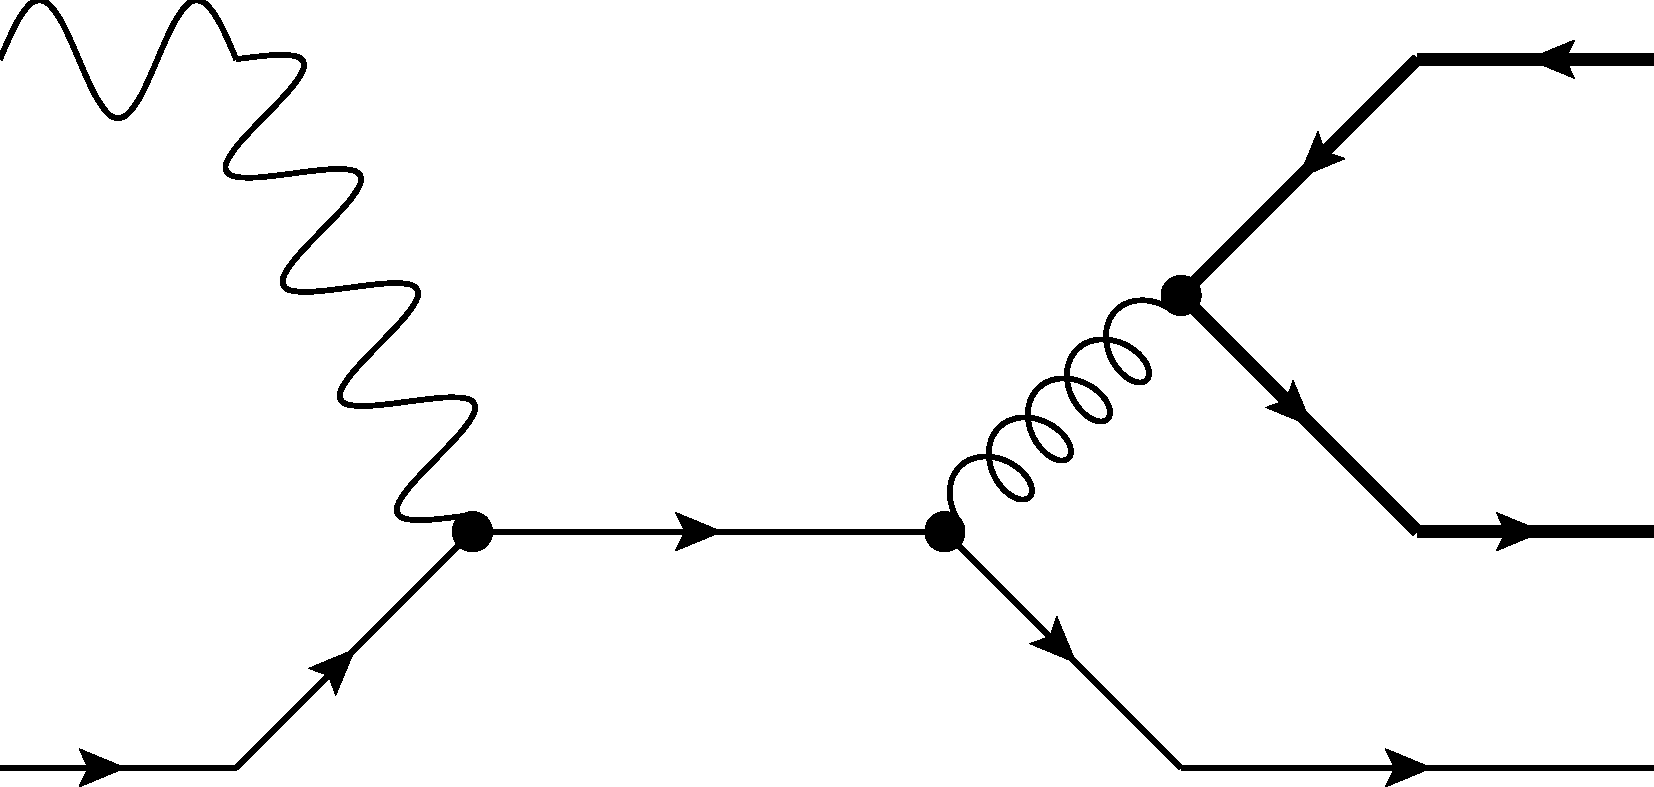
\includegraphics[width=.2\textwidth]{pyfeyn2/nlo-q-4} + 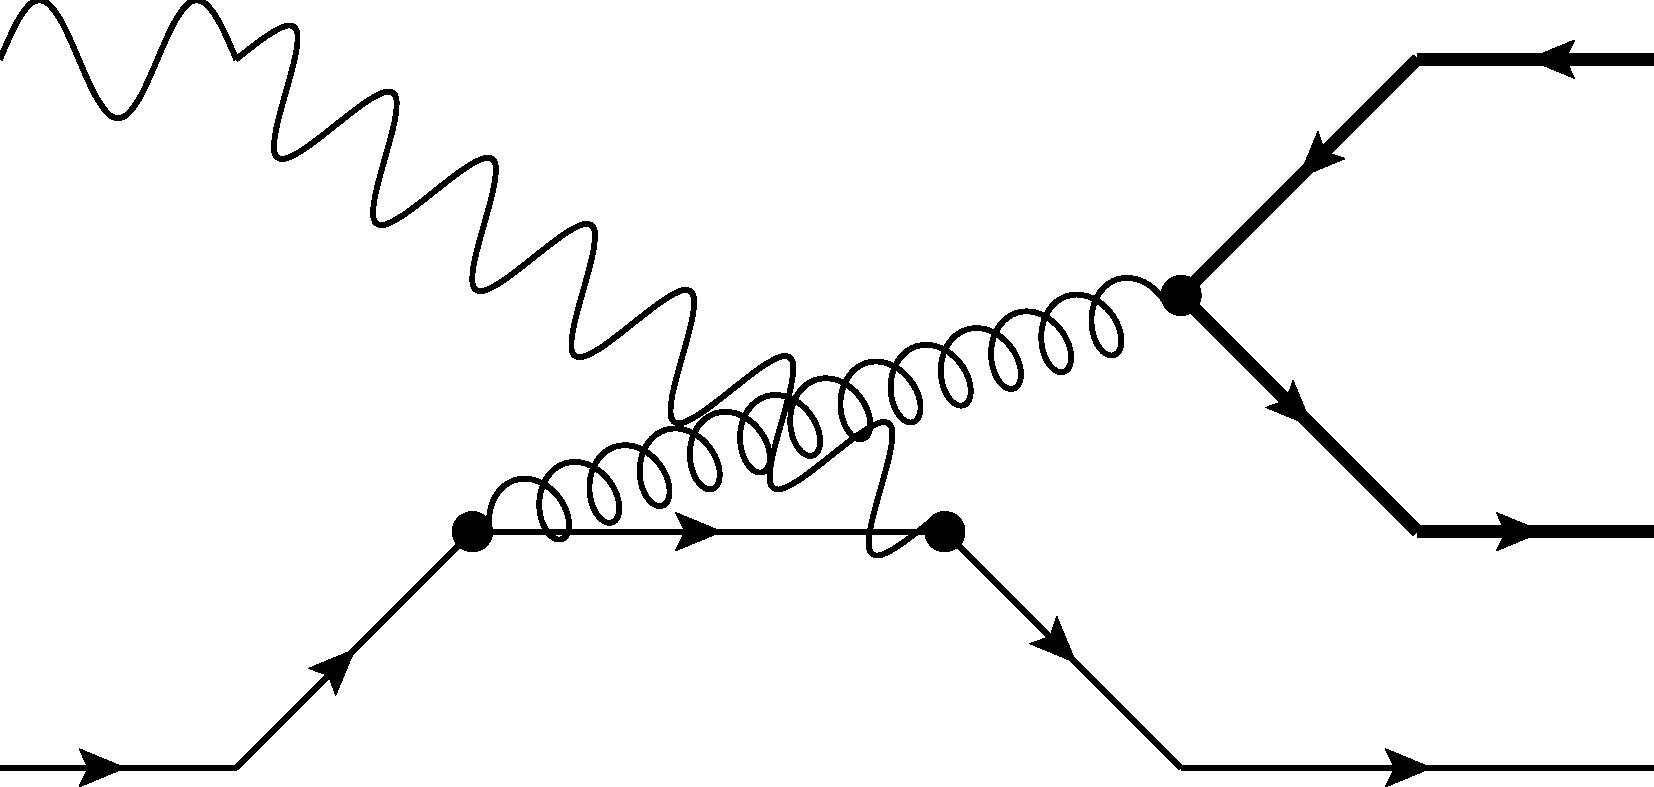
\includegraphics[width=.2\textwidth]{pyfeyn2/nlo-q-3}
\item $\Rightarrow 2xg_1(x) \sim e_L^2\cdot \xi\Delta f_u(\xi) \otimes d_{P,q}^{(1)}(\chi,\chi')$
\item $d_{P,q}^{(1)}(\chi,\chi') = c_1(\chi,\chi')\ln(\chi) + c_2(\chi,\chi')\DiLog\left(\frac{1+\chi'}{1+\chi}\right)+\ldots$ \checkmark
\item $\frac{m^2}{s} = \frac{\chi}{(1+\chi)^2}$ and $\frac{m^2}{s+Q^2} = \frac{m^2}{s'} = \frac{\chi'}{(1+\chi')^2}$ and $\frac{m^2}{Q^2} = \frac{\chi_q}{(1-\chi_q)^2}$
\end{itemize}
\end{frame}

\begin{frame}{Computation Review - Collinear Poles}
collinear poles appear as $1/\epsilon$ in

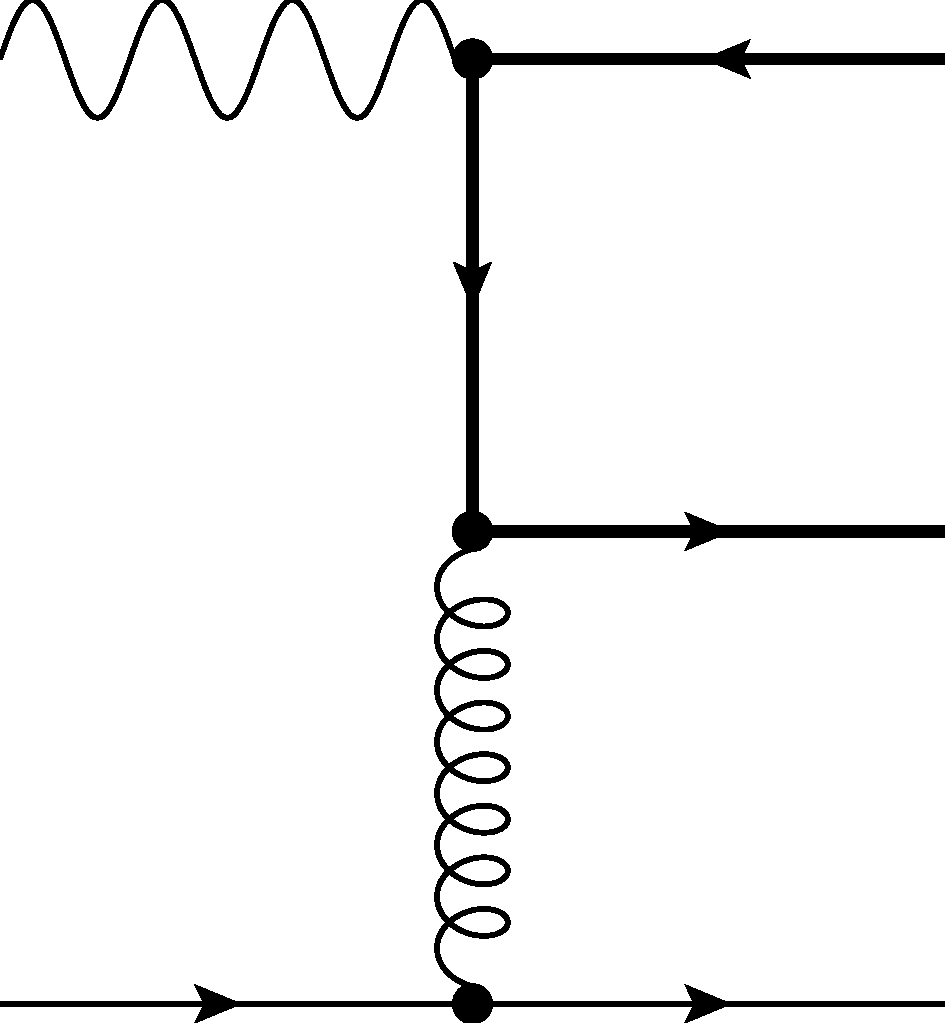
\includegraphics[width=.3\textwidth]{pyfeyn2/nlo-q-1} or 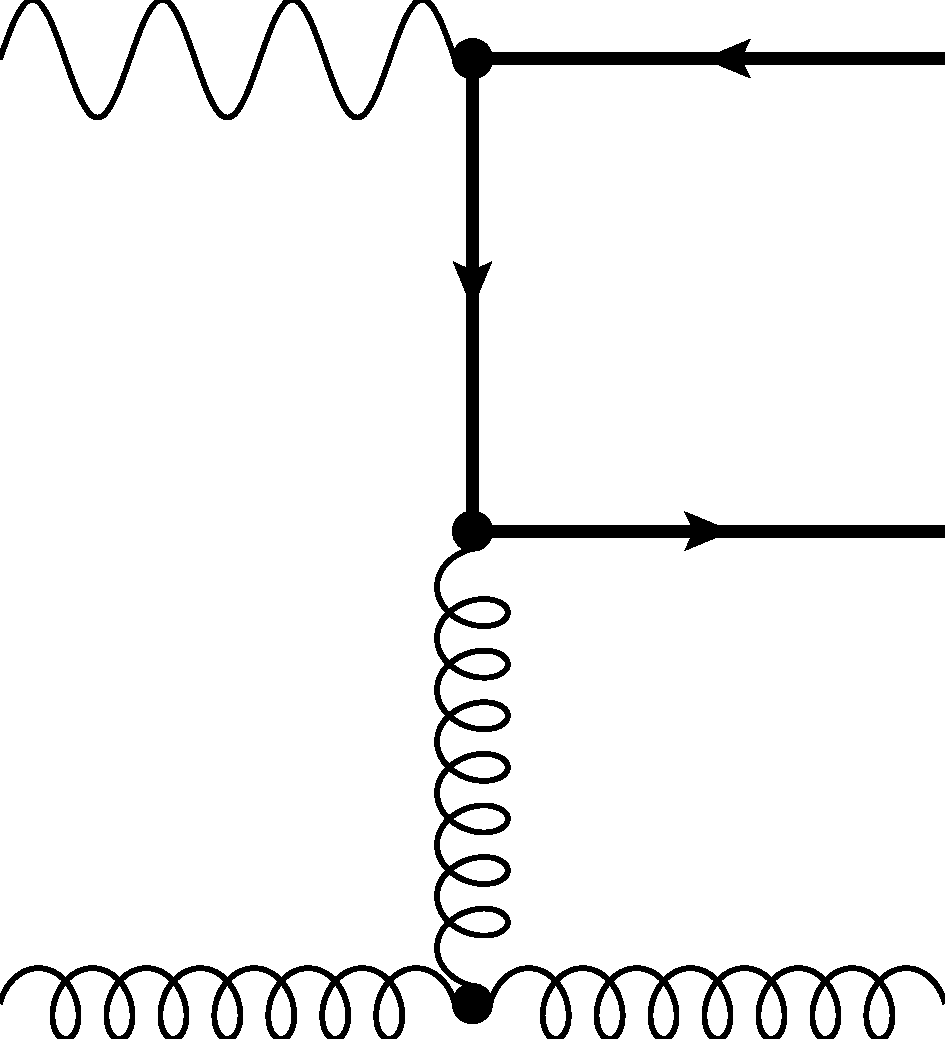
\includegraphics[width=.4\textwidth]{pyfeyn2/nlo-g-4}

\begin{itemize}
\item remove by mass factorization $\to \MSbar_m$
\item $\Rightarrow 2xg_1(x) \sim e_H^2\cdot \xi\Delta g(\xi) \otimes \ln(\mu_F^2/m^2) \bar c_{P,g}^{F,(1)}(\chi,\chi_q)$
\item $\bar c_{P,g}^{F,(1)}(\chi,\chi_q) = c_1(\chi,\chi_q)\ln(\chi) + c_2(\chi,\chi_q)\DiLog\left(\frac{1-\chi_q}{1+\chi}\right) + \ldots$ (\checkmark for $Q^2\gg m^2$ )
\end{itemize}
\end{frame}


\begin{frame}{Computation Review - Virtual and Soft Poles}
virtual diagrams are

\fxerror{insert diagrams}

soft poles appear in the limit of a soft gluon $k_2\rightarrow 0$

\fxerror{insert diagrams}

soft + virtual + renormalisation is finite!
\end{frame}
